\newpage
\subsection{Terraform}\label{implementierung_terraform}

\subsubsection{Terraform und AWS Setup}

Um das Projekt mit Terraform auf AWS zur Verfügung zu stellen muss zunächst Terraform und die AWS CLI installiert werden.
Terraform kann mit \hyperref[lst:terraform_setup]{ASDF} installiert werden.
Nach der Installation steht es als Kommandozeilen Tool zur Verfügung.
Mit ASDF lassen sich über Plugins verschiedene Versionen von Abhängigkeiten wie Erlang, Elixir, Terraform und Node.js verwalten.
\footnote{{ASDF Installation, vgl.~\cite{ASDF}}}

Die Installation der AWS CLI erfolgt über die \href{https://docs.aws.amazon.com/cli/latest/userguide/install-cliv2-linux.html}{Anleitungen von AWS} selbst.
Anschließend muss die CLI noch konfiguriert werden, dies wird über das Kommando \texttt{aws configure} gemacht. \\

Falls mehrere AWS Accounts über die CLI benutzt werden sollen, kann man separate Profile erstellen.
Dazu ruft man z.B. \texttt{aws configure --profile=kuffel} auf, um ein Profil mit dem Namen \texttt{kuffel} anzulegen. \\

AWS verwendet für die Authentifizierung und Autorisierung über die CLI sogenannte Access Keys, diese sind in einen \textsl{Access Key} und einen \textsl{Secret Access Key} unterteilt.
Sie sind immer einem IAM-Benutzer zugeordnet.
Es muss also zunächst ein neuer IAM-Benutzer angelegt werden.
Dazu meldet man sich mit dem Root Account (oder einem IAM Administrator Account) an der AWS Management Konsole an.

\begin{enumerate}
  \item Unter \textbf{Services} den Punkt \textbf{IAM} auswählen.
  \item Unter \textbf{Users} mit \textbf{Add User} einen neuen Benutzer erstellen.
  \item Der Benutzer benötigt \textbf{Programmatic Access}.
  \item Für die Verwendung mit Terraform benötigt der Benutzer die Policy \textbf{AdministratorAccess}.
  \item Die AWS Konsole zeigt anschließend den \textsl{Access Key} und einen \textsl{Secret Access Key} an diese sollten gesichert werden.
\end{enumerate}

Die AWS CLI kann im Anschluss mit \textbf{aws configure} eingerichtet werden die Region ist dabei \texttt{eu-central-1} und das Datenformat ist \texttt{JSON}.

Nachdem die CLI eingerichtet ist, kann der AWS Provider mit dem Profil konfiguriert werden.
Per Konvention legt man eine \hyperref[lst:terraform_main]{main.tf} an.
In dieser kann dann der AWS Provider und das AWS Profil angegeben werden.
Mit \texttt{terrafom init} können nun die Abhängigkeiten heruntergeladen werden und Terraform ist für die Verwendung mit AWS konfiguriert.

\paragraph{S3 Bucket für Terraform}

AWS S3 ist einer der ältesten AWS Dienste.
Er erlaubt das Ablegen von Dateien mit einem Pfad als Schlüssel in einem sogenannten Bucket.
Der Name eines Buckets ist global eindeutig und automatisch aus jeder AWS Region erreichbar.
\footnote{Create a Bucket, vgl.~\cite{AWS_S3}} \\

Terraform benutzt eine Datei um den Zustand der Terraform Konfiguration und den erstellten Ressourcen zu speichern.
Dieser \textbf{State} ist eine JSON Datei mit der Endung \textbf{.tfstate} und wird standardmäßig im gleichen Ordner wie die Konfiguration abgelegt.
Diese Datei könnte also auch über das Versionsverwaltungssystem verwaltetet werden,
was für die Arbeit im Team jedoch problematisch ist, da Änderungen von anderen Teammitgliedern auf anderen Branches zu Merge Konflikten führen könnten.
\footnote{Terraform State, vgl.~\cite{TERRAFORM_STATE}} \\

Um die Verwaltung des Zustandes in Umgebungen mit mehreren Teammitgliedern zu vereinfachen, bietet Terraform sogenannte \textbf{Backends} an.
\footnote{Terraform Backends, vgl.~\cite{TERRAFORM_BACKENDS}}

Für den AWS Provider bietet sich die Nutzung von S3 an.
Dafür muss zunächst ein S3 Bucket erstellt werden, das kann über die \hyperref[lst:terraform_s3_backend]{AWS CLI} durchgeführt werden.
Anschließend wird die \hyperref[lst:terraform_main]{main.tf} um einen Block erweitert, der beschreibt welcher Bucket und welche Datei von Terraform für den State verwendet werden soll.


\paragraph{Einrichtung ECR}

Im Verlauf der Arbeit werden die Docker Images aus dem CI/CD in eine Container Registry publiziert.
Auf AWS wird dafür die AWS Elastic Container Registry (ECR) verwendet.
Hier muss zunächst ein Repository angelegt werden.
\footnote{AWS ECR Creating a repository, vgl.~\cite{AWS_ECR_REPO_CREATE}}

Mit der AWS CLI lässt sich das mit einem \hyperref[lst:terraform_ecr_setup]{Kommando} erledigen. \\

Um die Terraform Skripte vor der Einrichtung der CI/CD Pipeline verifizieren zu können, benötigt man ein Image für die Ausführung auf AWS.
Dazu wird einfach mit dem Task \texttt{make docker} ein Image mit dem Tag \texttt{latest} erstellt und \hyperref[lst:terraform_docker_push]{manuell in das ECR} publiziert.


\newpage
\subsubsection{Terraform CLI}

\paragraph{Workspaces}

Durch Workspaces ist es möglich, ein und diesselbe Konfiguration für unterschiedliche Instanzen der Infrastruktur zu verwenden.
\footnote{Terraform Workspaces, vgl.~\cite{TERRAFORM_WORKSPACES}}
Die Workspaces werden als separater State im S3 Backend gespeichert.
Dies erlaubt Workspaces für Produktivumgebungen und Test- und Entwicklungszwecke voneinander zu trennen.
Die Verwaltung der Workspaces erfolgt über die Terraform CLI.
Auf diese Art kann die Duplizierung von IaC Code vermieden werden.
Das Kommando \texttt{terraform workspace list} listet alle aktuellen Workspaces auf.
Terraform Operationen werden immer auf dem aktuellen Workspace durchgeführt.
Um den Workspace zu wechseln wird das Kommando \texttt{terraform workspace select [NAME]`} benutzt.

Ein neuer Workspace lässt sich mit dem Kommando \texttt{terraform workspace new [NAME]} erstellen.
Dieser wird dann auch automatisch ausgewählt.

Workspaces lassen sich mit dem Kommando \texttt{terraform workspace delete [NAME]} löschen.
Terraform verweigert das Löschen von Workspaces in denen laut Statefile noch Ressourcen angelegt sind.
Dies kann mit einem Argument umgangen werden, führt jedoch dazu, dass diese Ressourcen sich nicht mehr über Terraform verwalten lassen und manuell entfernt werden müssen.

\paragraph{Variablen}

Workspaces sind vor allem dann sinnvoll, wenn die Terraform Konfiguration sich nur geringfügig je nach Workspace unterscheidet.
In den meisten Fällen geht es hier um Namen von Ressourcen oder DNS Einträgen.
Das kann über Variablen realisiert werden.
Diese werden per Konvention in einer separaten Datei mit dem Namen \hyperref[lst:terraform_variables]{variables.tf} definiert
\footnote{Terraform Variables, vgl.~\cite{TERRAFORM_VARIABLES}} \\

Grundsätzlich gibt es für die Überschreibung von Variablen in Terraform zwei Wege:

\begin{itemize}
  \item \textbf{Per Datei:} terraform plan -var="deployment\_name=ex-app"
  \item \textbf{Per Argument:} terraform plan -var-file=deployments/demo.tfvars
\end{itemize}

Die Überschreibung über eine Datei ist bei vielen Variablen sinnvoll und kann separat versioniert werden.

\paragraph{Plan, Apply, Destroy}

Die wichtigsten CLI Kommandos sind Plan, Apply und Destroy.
Diese zeigen entweder Änderungen an der Infrastruktur an, führen diese aus oder entfernen durch Terraform verwaltetet Infrastruktur.
Da diese Kommandos destruktiv sein können und bei falscher Handhabung zu Problemen führen können, sollte man sich mit diesen Kommandos vertraut machen.
\footnote{Terraform Provisioning, vgl.~\cite{TERRAFORM_RUN}} \\


Das Kommando \texttt{terraform plan} vergleicht die beschriebene Infrastruktur mit der aktuell im State gespeicherten und gibt die geplanten Änderungen aus.
\footnote{Terraform Plan, vgl.~\cite{TERRAFORM_PLAN}}

Diese Operation nimmt keine Veränderungen an der Infrastruktur von.
Sie kann verwendet werden um zu ermitteln welche Änderungen durchgeführt werden sollen.

Die Änderungen werden dabei folgendermaßen unterschieden:

\begin{itemize}
  \item \textbf{Create:} Ressourcen die neu erstellt werden (z.B. neuer Server).
  \item \textbf{In-Place Update:} Ressourcen die i.d.R. ohne Ausfall aktualisiert werden (z.B. neue Firewall Regel)
  \item \textbf{Destroy:} Ressourcen die entfernt werden.
\end{itemize}

Um sicherzustellen, dass der angezeigte Plan später auch mit dem \texttt{apply} genauso ausgeführt wird, kann man diesen in eine Datei schreiben lassen (\texttt{terraform plan -out=deployment.plan}).
Diese Datei kann für das Terraform Apply Kommando als Eingabe verwendet werden. \\

Das Kommando \texttt{terrafrom apply} verändert die Infrastruktur basierend auf der Konfiguration oder einem zuvor gespeicherten Plan.
\footnote{Terraform Apply, vgl.~\cite{TERRAFORM_APPLY}} \\

Die Ausgaben entsprechen denen des \textbf{terraform plan} Kommandos und müssen vor der Ausführung mit einer Eingabe bestätigt werden.
Zum Überspringen von Benutzereingaben und zur direkten Durchführung von Änderungen kann das Argument \texttt{-auto-approve} angegeben werden. \\

Das Kommando \texttt{terrafrom destroy} unterstützt die gleichen Parameter wie \textsl{Plan} und \textsl{Delete} und entfernt die von Terraform verwaltetet Infrastruktur vollständig.
\footnote{Terraform Destroy, vgl.~\cite{TERRAFORM_DESTROY}}

Dabei wird der State mit der Konfiguration abgeglichen, d.h. eine entfernte Regel in einer AWS Security Group, die im State noch vorhanden ist, wird ebenfalls entfernt.

\subsubsection{AWS Infrastruktur}

Für die Anwendung wird AWS ECS und Fargate verwendet.
Die Infrastruktur auf AWS sieht folgendermaßen aus:

\begin{figure}[htb]
  \centering
  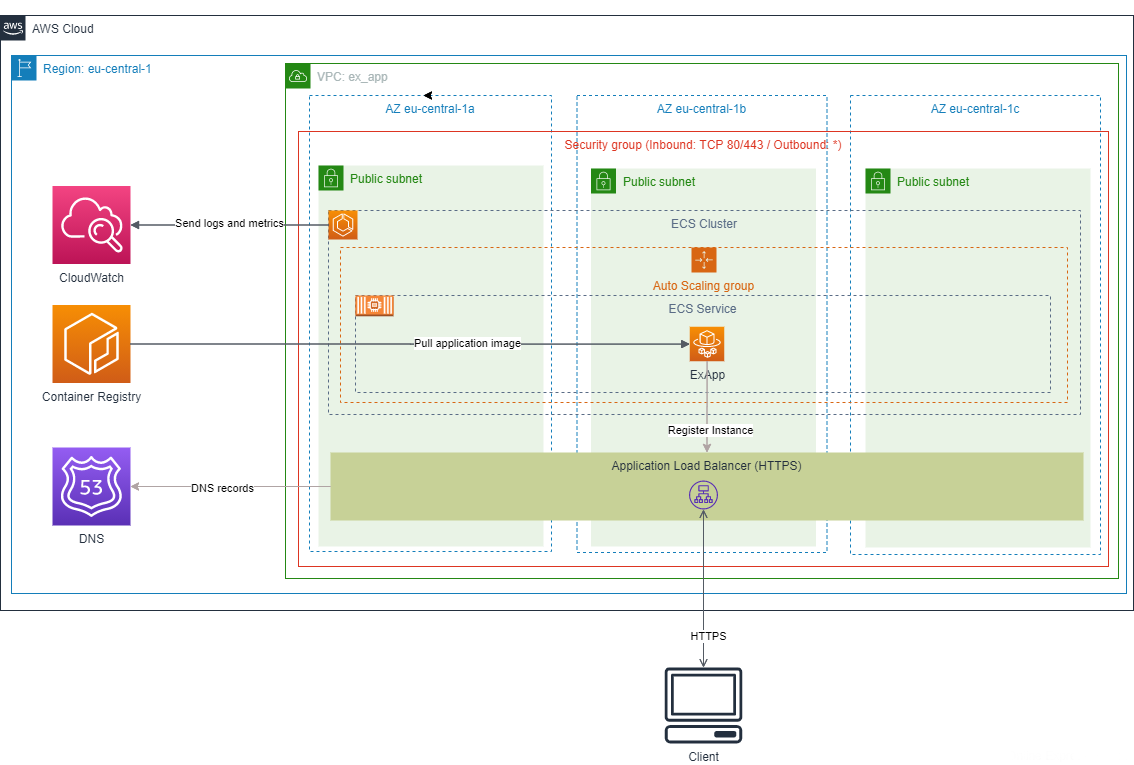
\includegraphics[width=1.0\textwidth]{images/aws_infrastruktur.png}
  \caption[AWS Infrastruktur]{AWS Infrastruktur}
  \label{fig:aws_infrastructure}
\end{figure}

\begin{itemize}
  \item Die Anwendung wird in der Region eu-central-1 (Frankfurt) installiert.
  \item Es wird eine eigene VPC mit Subnets in den drei verfügbaren AZs verwendet.
  \item Die Security Group erlaubt eingehenden Datenverkehr auf Port 80 (HTTP) und 443 (HTTPS).
  Der ausgehende Datenverkehr ist nicht beschränkt.
  \item Ein ECS Cluster der Instanzen in allen 3 Regionen starten kann wird für den ExApp Service verwendet.
  \item Der Cluster sendet Log-Ausgaben und Metriken (wie RAM/CPU Auslastung) an AWS CloudWatch.
  \item Die Images für die Tasks in dem ECS-Service werden aus der AWS Container Registry heruntergeladen.
  \item Wird ein Task gestartet, registriert er sich am Application Load-Balancer.
  Sobald der Healthcheck des Load-Balancers meldet, dass dieser auf HTTP-Anfragen antwortet, erhält der Task Traffic vom ALB.
  \item Der AWS Application Load-Balancer wird mit einem A- und AAAA-Record in Amazons Route 53 DNS registriert.
  \item Der Load-Balancer ist über HTTPS erreichbar und terminiert SSL, um die Anfragen an die jeweiligen Container weiterzuleiten.
  Clients rufen die URL vom Load-Balancer auf.
  \item Mittels AWS Metriken wird ermittelt, ob Tasks eine CPU Auslastung von > 50\% über einen Zeitraum von 60 Sekunden haben.
  Ist das der Fall werden bis zu 4 weitere Container gestartet, um die Last zu verteilen.
\end{itemize}

Die jeweiligen Terraform Skripte können beliebig unterteilt werden, die kompletten Skripte finden sich im Anhang dieser Arbeit.
Eine gängige Konvention bei der Benennung von Terraform Skripte ist diese einfach mit einer Nummer zu versehen.
Auch wenn Terraform die Reihenfolge bei der Erstellung der Ressourcen selbst ermittelt, so ist es doch hilfreich die Reihenfolge und Art der Ressourcen auf diese Art und Weise zu gruppieren.

\paragraph{VPC}

Jede Installation der Anwendung läuft in einer separate \hyperref[lst:terraform_vpc]{VPC} mit einem eigenen Internet Gateway und einer Route Table.
Der CIDR der VPC ist immer 172.16.1.0/24.
Die jeweiligen Subnetze sind über mehrere AZs verteilt und unterstützen bis zu 254 Adressen.

In der Region Frankfurt (eu-central-1) können somit insgesamt 762 Container über alle drei Subnetze verteilt verwendet werden.

\paragraph{Security Groups}

Mit \hyperref[lst:terraform_security_group]{Security Groups} werden die Firewall Regeln für eine \hyperref[lst:terraform_vpc]{VPC} und ihre Subnetze dargestellt.
Die Anwendung erlaubt hierfür eingehenden Datenverkehr auf Port 80 HTTP und 443 HTTPS.
Ausgehender Datenverkehr und Datenverkehr innerhalb der VPC ist ebenfalls erlaubt.

\paragraph{ECS}

Für die Anwendung wird AWS Elastic Container Service ECS verwendet.
Dafür muss ein entsprechender \hyperref[lst:terraform_ecs]{ECS Cluster} definiert werden.
Diesem Cluster sind keine Server zugeordnet und er verursacht dadurch keine zusätzlichen Kosten.

Für AWS Fargate wird hier noch zusätzlich eine \hyperref[lst:terraform_fargate_role_policy]{IAM Policy} definiert.
Diese erlaubt den Zugriff auf ECR für die Docker Images und CloudWatch für die Logs.


\paragraph{Task und Service}

ECS unterscheidet zwischen Tasks und Services.
Ein Service besteht aus einem oder mehreren Tasks der gleichen Task-Definition.
Für die Task-Definition wird eine \hyperref[lst:terraform_ecs_task_json]{JSON Datei} erstellt, dort werden die Docker Einstellungen des Containers vorgenommen.

Es lassen sich auch mehrere Container innerhalb einer Task-Definition starten und konfigurieren.
Wird ein als \textbf{Essential} markierter Container beendet, so wird der gesamte Task von AWS neu gestartet.

Aus einer Task-Definition wird ein \hyperref[lst:terraform_ecs_task]{Task} erstellt.
Dieser wird dann in einem Service gestartet.
Bei der Definition des Services wird auch angegeben, wie viele Instanzen von einem Task in einem Service gestartet werden sollen.


\paragraph{Autoscaling}

Mit \hyperref[lst:terraform_autoscaling]{Autoscaling} kann man automatisch mehrere Tasks starten lassen, wenn bestimmte Bedingungen erfüllt sind.
Die aktuelle Konfiguration überwacht die CPU Auslastung, liegt diese über einen Zeitraum von 60 Sekunden bei mehr als 50\%, wird ein zusätzlicher Task innerhalb des Services gestartet.
Dabei werden maximal 4 Instanzen eines Tasks gestartet.
Fällt die CPU Last unter 50\% werden die Tasks automatisch entfernt.
Es lassen sich beliebige Metriken aus AWS CloudWatch verwenden.
Auf diese Art und Weise kann man eine Anwendung automatisch skalieren.

\paragraph{Application Load-Balancer}

Die Anwendung verwendet einen \hyperref[lst:terraform_alb]{AWS Load-Balancer}.
Hierfür wird der Application-Load-Balancer für HTTP und HTTPS verwendet.

Der ALB verwendet Target-Groups, um die ECS Fargate-Tasks anzusprechen.
Hier befindet sich auch ein Health-Check der periodisch eine Anfrage an die Tasks sendet.
Werden diese Anfragen mit einem HTTP Status Code kleiner als 500 beantwortet, so wird dieser Task weiterhin Traffic von dem Load-Balancer erhalten.

Der ALB hat zwei Listener.
Einen für HTTP der die Anfragen auf HTTPS umleitet und den HTTPS Listener.
Der HTTPS Listener verwendet ein Wildcard Zertifikat von AWS (*.kuffel.me) und terminiert den SSL Verkehr in Richtung der Tasks.

Der ALB regelt die Verteilung des Traffics und die Tasks melden sich an dem ALB an und ab.
Wenn ein ECS Task beendet wird, hört der ALB auf diesem weitere Anfragen zu senden.

Bei einem Update der Container bleibt die Anwendung jederzeit verfügbar.
Alte Container bekommen so lange Anfragen bis die neuen Container am ALB registriert sind.
Anschließend werden diese am ALB abgemeldet und von ECS beendet.

\paragraph{DNS}

Der ALB hat einen CNAME im AWS eigenen DNS Route 53, an dem Load-Balancer hängt ein Wildcard Zertifikat, dieses würde mit dem ALB CNAME von keinem Browser akzeptiert.
Über Route 53 wird ein \hyperref[lst:terraform_dns]{Alias für den CNAME} des ALB eingetragen.
Dazu wird ein A-Record für IPv4 und ein AAAA-Record für IPv6 verwendet.
Um Route 53 verwenden zu können empfiehlt es sich ein eigene Hosted Zone mit einer eigenen Domain anzulegen.
Diese kann über die AWS Route 53 Konsole reserviert werden.

\paragraph{Sonstige Dateien}

Alle Ausgaben der Container werden nach AWS CloudWatch umgeleitet.
Dafür benötigt man eine \hyperref[lst:terraform_monitoring]{AWS Log Group}.
Diese wird ebenfalls über Terraform erstellt.
Über Cloud Watch Filter Metrics können Alarme erstellt werden, die beim Auftreten bestimmter Texte in den Logs zu einer Benachrichtigung führen.
Logs werden nach 30 Tagen automatisch wieder gelöscht.

Alle Terraform Dateien verwenden Variablen und Workspaces, um die jeweiligen Installationen voneinander zu trennen.
Die verwendeten Variablen und ihre Standardwerte werden in der \hyperref[lst:terraform_variables]{variables.tf} definiert.
Nur Variablen, die in der variables.tf definiert sind, können überschrieben werden.

Nach der Ausführung von Terraform werden neue Ressourcen angelegt.
Die Namen dieser Ressourcen sind nicht immer vorhersehbar.
Um eine Ausgabe der angelegten Ressourcen nach der Ausführung zu steuern, kann eine \hyperref[lst:terraform_output]{outputs.tf} verwendet werden.
